\documentclass[11pt]{beamer}
\mode<presentation>
\let\Tiny=\tiny
\usetheme{CambridgeUS}
\usefonttheme{professionalfonts}
\usepackage[brazil]{babel}
\usepackage[utf8]{inputenc}
\usepackage{ucs}
\usepackage{amsfonts}
\usepackage{amssymb}
\usepackage{amsmath}
\newtheorem{mydef}{Definição}
\newtheorem{myexample}{Exemplo}
\usepackage{pbox}
\usepackage{multirow}

\title{Métodos Ágeis}
\author{}
\date{}

\begin{document}

    \begin{frame}[plain]
        \titlepage
    \end{frame}

   \section{Métodos Ágeis}

    \begin{frame}{Métodos Ágeis}
      \begin{itemize}
         \item Um ponto importante para o sucesso de um produto de \textit{software} é ser lançado antes da concorrência.
         \item Por si, não garante o sucesso, mas é sabido que os clientes hesitam em trocar um produto que já usam por outro recente.
      \end{itemize}
    \end{frame}

    \begin{frame}{Métodos Ágeis}
      \begin{itemize}
         \item A partir dos anos 90 surge insatisfação com o desenvolvimento orientado a planos, levando à criação dos métodos ágeis.
         \item Esta nova abordagem, com o seu desenvolvimento mostrou ser a que melhor permite entregar \textit{software} com tamanha restrição de tempo e atendendo a outros parâmetros como custo e confiabilidade, além de lidar de maneira mais fácil com as mudanças.
      \end{itemize}
    \end{frame}

    \begin{frame}
      \frametitle{Manifesto Ágil}

      \textbf{Manifesto para o desenvolvimento ágil de software}

      ``Estamos descobrindo maneiras melhores de desenvolver software, fazendo-o nós mesmos e ajudando outros a fazerem o mesmo. Através deste trabalho, passamos a valorizar:
\\
      \begin{center}
        \textbf{Indivíduos e interações} mais que processos e ferramentas\\
        \textbf{Software em funcionamento} mais que documentação abrangente\\
        \textbf{Colaboração com o cliente} mais que negociação de contratos\\
        \textbf{Responder a mudanças} mais que seguir um plano\\
      \end{center}

      Ou seja, mesmo havendo valor nos itens à direita, valorizamos mais os itens à esquerda.''

      \begin{table}
        \resizebox{\textwidth}{!}{%
          \begin{tabular}{l l l l}
          Kent Beck        &Mike Beedle   &Arie van Bennekum &Alistair Cockburn\\
          Ward Cunningham  &Martin Fowler &James Grenning    &Jim Highsmith\\
          Andrew Hunt      &Ron Jeffries  &Jon Kern          &Brian Marick\\
          Robert C. Martin &Steve Mellor  &Ken Schwaber      &Jeff Sutherland\\
          Dave Thomas      &              &                  &
        \end{tabular}}
      \end{table}
    \end{frame}

    \begin{frame}{Métodos Ágeis}
      Os métodos ágeis possuem alguns princípios:
      \begin{itemize}
         \item entrega incremental e contínua (modelo iterativo incremental);
         \item envolvimento do cliente;
         \item foco nas pessoas, e não no processo;
         \item adaptabilidade a mudanças;
         \item atenção à qualidade e uso de técnicas de excelência;
         \item simplicidade $\rightarrow$ redução de complexidade do sistema.
      \end{itemize}
    \end{frame}
    
    \begin{frame}{Métodos Ágeis}
      Riscos:
      \begin{itemize}
         \item cliente não participar do processo;
         \item não envolvimento dos membros do time;
         \item dificuldade em priorizar mudanças devido a conflitos entre \textit{stakeholders};
         \item dificuldade em manter a simplicidade;
         \item resistência das organizações em adaptar seus processos.
      \end{itemize}
    \end{frame}

    \begin{frame}
      \frametitle{Ágil $\times$ Rápido}
      \begin{itemize}
         \item Ágil significa dar respostas rapidamente às mudanças.
         \item Os metodos ágeis não garantem que o \textit{software} será entregue em menos tempo.
         \item Mas visam garantir que o processo se adaptará melhor às mudanças. 
      \end{itemize}
    \end{frame}

    \begin{frame}{Métodos Ágeis $\times$ Métodos Orientados a Planos}
      \begin{itemize}
         \item Os métodos orientados a planos, geralmente, exigem grande burocracia.
         \item Por exemplo, um projeto pode estar avaliado em 40\% de conclusão, porém nada foi implementado.
         \item Nos métodos ágeis, o esforço de documentação é substituído, em parte, pela criação do \textit{software}.
      \end{itemize}
    \end{frame}

    \begin{frame}
      \frametitle{Documentação}
      \begin{itemize}
         \item Documentação extensa não garante que não haverá mudanças.
         \item Pelo contrário, as mudanças levarão à reescrita da documentação.
         \item Se não devidamente alterada, criará inconsistência entre documentação e \textit{software} implementado.
      \end{itemize}
    \end{frame}

    \begin{frame}
      \frametitle{Documentação}
      \begin{itemize}
         \item Os métodos ágeis, no entanto, não são caóticos. Eles estabelecem, e necessitam de regras bem definidas e disciplina ao cumpri-las.
         \item A documentação, nos métodos ágeis, só é criada quando agrega valor.
         \item Um exemplo de documentação com altíssimo valor agregado é os códigos de teste automatizado. 
      \end{itemize}
    \end{frame}

    \begin{frame}
      \frametitle{Planejamento}
      \begin{itemize}
         \item A gerência de projetos tradicional estabelece planejamento detalhado tanto a curto quanto a médio e longo prazo.
         \item Já na gerência de projetos ágeis, o detalhamento é feito apenas no planejamento de curto prazo. No médio prazo, é feito um planejamento de alto nível e, no longo prazo, é esboçada somente a visão do que espera-se ser atingido.
         \item Deste modo, as respostas às mudanças são mais rápidas e geram menos impacto (retrabalho). 
      \end{itemize}
    \end{frame}

    \begin{frame}{Métodos Ágeis}
      \begin{itemize}
         \item Há diversos métodos ágeis.
         \item Dentre estes, os mais famosos são o eXtreme Programming (XP) e o Scrum.
      \end{itemize}
    \end{frame}
    
    \section{XP}

    \begin{frame}{eXtreme Programming}
      O XP compreende as seguintes práticas:
      \begin{itemize}
        \item programação em pares;
        \item desenvolvimento orientado a testes (TDD);
        \item planejamento incremental;
        \item cliente no local;
        \item refatoração;
        \item integração contínua;
        \item pequenos \textit{releases};
        \item projeto simples;
        \item padrões de codificação;
        \item propriedade coletiva do código;
        \item metáfora do sistema;
        \item semana de trabalho de 40 horas.
      \end{itemize}
    \end{frame}

    \begin{frame}{Programação em pares}
      \begin{itemize}
         \item Na programação em pares, dois programadores trabalham na mesma estação de trabalho.
         \item Um programador fica como "piloto", trabalhando diretamente no teclado.
         \item O outro programador fica como "copiloto", auxiliando o primeiro.
      \end{itemize}
    \end{frame}

    \begin{frame}{Programação em pares}
      Henrik Kniberg, no livro Scrum and XP from the Trenches (2ed.) fala das seguintes conclusões que teve ao utilizar programação em pares:
      \begin{itemize}
         \item melhora na qualidade do código;
         \item melhora o foco da equipe no escopo;
         \item a resistência à prograamação em pares tem motivação no fato de muitos programadores nunca terem experimento-a;
         \item é exaustiva e não deve ser utilizada todos os dias;
         \item alguns programadores não ficam confortáveis com esta prática;
         \item revisão de código é uma alternativa válida à programação em pares;
         \item o copiloto (ou navegador) deve ter um computador à disposição para consultar documentação, etc.;
         \item não deve ser forçada à equipe.
      \end{itemize}
    \end{frame}

    \begin{frame}{Desenvolvimento orientado a testes (TDD)}
      \begin{itemize}
         \item No desenvolvimento dirigido a testes, testes e desenvolvimento são realizados de maneira intercalada.
         \item O código e desenvolvido de maneira incremental e sempre para corrigir uma falha em um teste.  
      \end{itemize}
    \end{frame}

    \begin{frame}
      \frametitle{\textit{Test Driven Development}}
      \begin{figure}[ht]
        \centering
        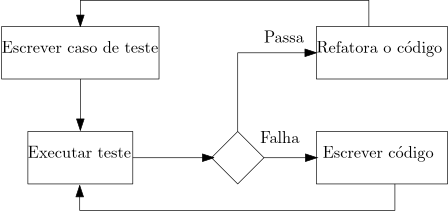
\includegraphics[height=4cm, width=9cm]{figures/fluxo_tdd.png}
      \end{figure}\footnote{Na refatoração o código deve obviamente passar nos testes.}
    \end{frame}

    \begin{frame}{Desenvolvimento orientado a testes (TDD)}
      Henrik Kniberg, faz algumas ponderações sobre o TDD:
      \begin{itemize}
         \item TDD é difícil de aprender, porém "viciante";
         \item efeitos profundos no desenho do sistema;
         \item demora para colocar em novo produto, porém com rápido retorno sobre investimento;
         \item garantir o tempo necessário para escrever testes fáceis (ferramentas corretas, educação, prover as classes utilitárias e base certas).
         \item garantir que cada \textit{feature} chave tem ao menos um teste de aceitação fim-a-fim;
         \item garantir que qualquer código complexo ou crítico é coberto por testes de unidade;
         \item saber exatamente qual parte do código não está coberta por testes;
         \item não deixar para escrever testes depois.
      \end{itemize}
    \end{frame}

    \begin{frame}{Planejamento incremental}
      \begin{itemize}
         \item No XP, assim como nos demais métodos ágeis, o planejamento deve ser realizado incrementalmente.
         \item Decisões de desenho e organização devem ser realizadas de acordo com a necessidade.
      \end{itemize}
    \end{frame}

    \begin{frame}{Cliente no local}
      \begin{itemize}
         \item O XP espera maior envolvimento do cliente.
         \item Cliente aqui significa aquele que define os requisitos.
         \item Para o desenvolvimento de produto de \textit{software}, onde o responsável pelos requisitos (gerente de produto) faz parte da empresa desenvolvedora, esta parte é facilitada.
         \item Para o desenvolvimento de projeto de \textit{software} pode ser mais complicado um maior envolvimento do cliente.
      \end{itemize}
    \end{frame}

    \begin{frame}{Refatoração}
      \begin{itemize}
         \item Refatoração é a reescrita de código com o intuito de melhorá-lo.
         \item Um código melhor geralmente significa código mais legível.
         \item Outros elementos presentes na refatoração de código são:
         \begin{itemize}
          \item a eliminação de funções, classes e objetos desnecessários;
          \item divisão de funções em mais funções;
          \item uso de padrões de projeto e melhorias de arquitetura;
          \item outros.
         \end{itemize}
      \end{itemize}
    \end{frame}

    \begin{frame}{Integração contínua}
      \begin{itemize}
         \item Toda nova entrega deve integrar-se ao \textit{software} já entregue.
         \item Ao subir o novo código ao repositório, o sistema de integração contínua faz seu \textit{build} automático, executa testes automatizados e realiza o \textit{deploy}.
         \item Alguns sistemas não fazem o \textit{deploy} automatizado. Para estes casos, os sistemas geralmente entregam o pacote já pronto para que o \textit{deploy} seja feito.
         \item Acaba com o problema do "na minha máquina funciona".
      \end{itemize}
    \end{frame}

    \begin{frame}{Pequenos \textit{releases}}
      \begin{itemize}
         \item O método ágil pressupõe um modelo interativo incremental, então faz sentido que as \textit{releases} sejam pequenas.
         \item Assim, haverá mais entregas e consequentemente mais testes e mais \textit{feedback} dos usuários. 
      \end{itemize}
    \end{frame}    

    \begin{frame}{Projeto simples}
      \begin{itemize}
         \item Não apenas o código deve ser simples e sempre refatorado, mas o projeto como um todo.
         \item Deve-se sempre escolher soluções que diminuam a complexidade.
      \end{itemize}
    \end{frame}

    \begin{frame}{Padrões de codificação}
      \begin{itemize}
         \item Em projetos onde há mais de um desenvolvedor, é interessante que a organização defina um padrão de codificação.
         \item Isto significa que os códigos desenvolvidos pelos mais diferentes programadores serão de mais fácil entendimento pelos demais.
         \item Evita-se assim o problema de pedaços de código onde só um determinado programador sabe mexer.
      \end{itemize}
    \end{frame}

    \begin{frame}{Propriedade coletiva do código}
      \begin{itemize}
         \item O XP estabelece que não há propriedade de parte do código por um determinado programador.
         \item Toda a equipe é "dona" do código e pode modificá-lo.
         \item O Spotify utiliza modelo de "\textit{internal open source}" onde os desenvolvedores podem propor códigos aos mais diferentes projetos da empresa através de um servidor interno de
      \end{itemize}
    \end{frame}

    \begin{frame}{Metáfora do sistema}
      \begin{itemize}
         \item A comunicação entre clientes e desenvolvedores devem ser o mais simples o possível.
         \item No livro Extreme Programming Explained, Kent Beck define metáfora do sistema como "uma estória que qualquer um - clientes, programadores e gerentes - podem contar sobre o funcionamento do programa".
      \end{itemize}
    \end{frame}

    \begin{frame}{Semana de trabalho de 40 horas}
      \begin{itemize}
         \item Quando se fala de semana de trabalho de 40 horas o importante não é apenas a quantidade de horas, mas a qualidade destas horas.
         \item Muitas reuniões, retrabalho e falhas de comunicação podem impedir que os programadores trabalhem da melhor maneira.
         \item Como a produção de \textit{software} de alta qualidade é um trabalho mental, simplesmente colocar mais horas também não resolverá problema algum.
      \end{itemize}
    \end{frame}

   \section{Scrum}

    \begin{frame}{Scrum}
      \begin{itemize}
        \item O Scrum é método ágil que define um \textit{framework} para a organização de um projeto ágil.
        \item Diferente do XP, por exemplo, o Scrum não se baseia em um conjunto de técnicas, mas em definir papéis, artefatos,eventos e regras.
        \item Segundo Henrik Kniberg, no Scrum original, Jeff Sutherland utilizava as técnicas do XP, mas foi convencido por Ken Schwarber a manter o modelo mais simples, colocando a responsabilidade das equipes em escolher o que deveriam usar. 
      \end{itemize}
    \end{frame}
    
    \begin{frame}{Scrum}
       O Scrum define os seguintes papéis:
       \begin{itemize}
         \item \textit{Development Team};
         \item \textit{Scrum Master};
         \item \textit{Product Owner}.
      \end{itemize}
    \end{frame}

    \begin{frame}{\textit{Development Team}}
      \begin{itemize}
         \item auto-organizável $\rightarrow$ toma as decisões de como transformar o \textit{Product Backlog} (conjunto de requisitos) em um produto funcional;
         \item possui todas as características, como um time, necessárias para criar um incremento do produto;
         \item todos são chamados de desenvolvedores independente do trabalho que realizam;
         \item não há sub-times;
         \item possui entre 3 e 7 integrantes (sem incluir o \textit{Scrum Master} e o \textit{Product Owner}).
      \end{itemize}
    \end{frame}

    \begin{frame}{\textit{Scrum Master}}
      \begin{itemize}
         \item O \textit{Scrum Master} é o guardião das regras do \textit{Scrum} e responsável por garantir o respeito às mesmas.
         \item Faz a ligação entre o time, o \textit{Product Owner} e o público externo.
      \end{itemize}
    \end{frame}

    \begin{frame}{\textit{Product Owner}}
      \begin{itemize}
         \item Responsável por decidir quais funcionalidades serão implementadas e em qual ordem.
         \item Responsável por gerenciar o \textit{Product Backlog} (conjunto de requisitos).
      \end{itemize}
    \end{frame}

    \begin{frame}{Artefatos do \textit{Scrum}}
      Os artefatos utilizados pelo \textit{Scrum} são:
      \begin{itemize}
         \item \textit{Product Backlog};
         \item \textit{Sprint Backlog}.
      \end{itemize}
    \end{frame}

    \begin{frame}{\textit{Product Backlog}}
      \begin{itemize}
         \item O \textit{Product Backlog} é lista priorizada contendo os requisitos e características do produto a ser implementado.
         \item Ele nunca está completo e é alterado a medida que se vai entendo o que será construído.
         \item Pode ser utilizado por múltiplos times que estejam construindo o mesmo produto.
         \item O \textit{Product Owner} é o dono do \textit{Product Backlog}.
      \end{itemize}
    \end{frame}

    \begin{frame}{\textit{Product Backlog}}
      Um \textit{Product Backlog} pode conter:
      \begin{itemize}
         \item características;
         \item funcionalidades;
         \item recursos;
         \item \textit{bugs};
         \item entre outros.
      \end{itemize}
    \end{frame}

    \begin{frame}{\textit{Product Backlog}}
      Os itens do \textit{Product Backlog} são divididos em:
      \begin{itemize}
         \item a fazer;
         \item em execução;
         \item prontos.
      \end{itemize}
    \end{frame}

    \begin{frame}{\textit{Product Backlog}}
      Cada \textit{Product Backlog Item} (PBI) pode ter os seguintes campos:
      \begin{itemize}
         \item identificador;
         \item nome;
         \item importância;
         \item estimativa;
         \item estado.
      \end{itemize}
      Outros campos podem ser incluídos se necessários.
    \end{frame}

    \begin{frame}{\textit{Product Backlog}}
      \begin{table}
        \begin{tabular}{|l|l|l|l|l|l|}
          \hline
          ID & nome                                                                                          & imp. & estim. &estado\\
          \hline
          36 &\pbox{3.8cm}{Enquanto vendedor, desejo listar as vendas do último mês para ter um controle contábil.} & 21   & 2    &a fazer\\
          \hline          
          5  &\pbox{3.8cm}{Enquanto cliente, desejo inserir itens no carrinho para comprá-los.}                     & 34   & 65   &em execução\\
          \hline
          16 &\pbox{3.8cm}{Adaptar a \textit{interface} de usuário para cegos.}                                     & 8    & 34   &a fazer\\
          \hline
          3  &\pbox{3.8cm}{Criptografar os dados bancários.}                                                         & 34   & 21   &feito\\
          \hline
        \end{tabular}
      \end{table}
    \end{frame}
    
    \begin{frame}{\textit{Sprint Backlog}}
      \begin{itemize}
         \item O \textit{Sprint Backlog} é criado a partir do \textit{Product Backlog}.
         \item O dono do \textit{Sprint Backlog} é o \textit{Development Team}.
         \item Ele define as atividades que serão realizadas para que um determinado PBI seja implementado/realizado.
      \end{itemize}
    \end{frame}

    \begin{frame}{\textit{Sprint Backlog}}
      \begin{table}
        \begin{tabular}{|l|l|l|l|l|l|}
          \hline
          ID                  & nome                                                                                                &tarefa  &resp. &estim &estado \\
          \hline
          \multirow{5}{.05cm}{36} &\multirow{5}{*}{\pbox{3.5cm}{Enquanto vendedor, desejo listar as vendas do último mês para ter um controle contábil.}} &criar \textit{interface} &Phelipe &16h &feito\\
          \cline{3-6}
                              &                                                                                                           &implem. banco &Cleisson &12h &feito\\
                              \cline{3-6}
                              &                                                                                                           &implem. código &Diêgo &6h &feito\\
                              \cline{3-6}
                              &                                                                                                           &criar \textit{thumbnails} &Jesse &4h &feito\\
                              \cline{3-6}
                              &                                                                                                           &corrig. msg. erro &Mário &2h &exec.\\
          \hline          
        \end{tabular}
      \end{table}
    \end{frame}

    \begin{frame}{Scrum}
      \begin{itemize}
         \item O Scrum é o modelo iterativo incremental implementado de maneira radical.
         \item Isto significa que o processo de desenvolvimento utilizando Scrum é dividido em iterações, chamadas \textit{Sprints}.
          \item Cada \textit{Sprint} tem um tempo definido (entre 2 e 4 semanas).
      \end{itemize}
    \end{frame}

    \begin{frame}{Sprint}
       \begin{itemize}
          \item Toda \textit{Sprint} tem um objetivo e terá sempre como resultado \textit{software} funcional, um protótipo ou um desenho arquitetural.
          \item No caso do primeiro, este \textit{software} deve já estar integrado ao que foi feito anteriormente e deve ser colocado em ambiente de produção.
          \item Protótipos e desenhos arquiteturais servem para embasar \textit{sprints} futuras.
       \end{itemize}
    \end{frame}
    
    \begin{frame}{Sprint}
       As \textit{Sprints} podem ser de três tipos:
       \begin{itemize}
          \item funcional $\rightarrow$ quando seu objetivo é implementar funcionalidades para o usuário final;
          \item performance e confiabilidade $\rightarrow$ quando seu objetivo é melhorar performance, segurança, confiabilidade e eficiência do sistema;
          \item suporte $\rightarrow$ quando seu objetivo é atividades auxiliares, como desenvolver \textit{software} de infraestrutura ou projetar a arquitetura do sistema.
       \end{itemize}
    \end{frame}    

    \begin{frame}{\textit{Sprint}}
      Durante uma \textit{Sprint}:
      \begin{itemize}
         \item não há mudanças que ameacem os objetivos da \textit{Sprint};
         \item metas de qualidade não diminuem;
         \item o escopo pode ser clarificado e renegociado entre o \textit{Product Owner} e o time (se necessário).
      \end{itemize}
    \end{frame}

    \begin{frame}{\textit{Sprint Planning}}
      \begin{itemize}
         \item O pontapé inicial da \textit{Sprint} é chamado \textit{Sprint Planning}.
         \item É realizado em, no máximo, 8 horas (para uma \textit{Sprint} de 4 semanas) e envolve a equipe toda.
         \item Deve tratar 2 tópicos:
           \begin{itemize}
              \item o que pode ser feito nesta \textit{Sprint}?
              \item como o trabalho escolhido será realizado?
           \end{itemize}
      \end{itemize}
    \end{frame}
    
    \begin{frame}{\textit{Daily Scrum}}
      \begin{itemize}
         \item Durante cada dia de trabalho é realizado, no seu início, o \textit{Daily Scrum}. 
         \item O \textit{Daily Scrum} é uma reunião de 15 minutos entre o time de desenvolvimento e o \textit{Scrum Master} com o intuito de sincronizar o trabalho e planejá-lo para as próximas 24 horas.
      \end{itemize}
    \end{frame}

    \begin{frame}{\textit{Daily Scrum}}
      \begin{itemize}
         \item A reunião é realizada em pé e cada integrante diz o que fez no dia anterior e o que fará neste.
         \item Quando um membro do time possui algum problema, ele o trás ao restante dos integrantes, mas na reunião não é discutido como será resolvido.
         \item A solução será discutida após a reunião e apenas entre as pessoas que realmente possam resolvê-lo.
      \end{itemize}
    \end{frame}

    \begin{frame}{\textit{Sprint Review}}
      \begin{itemize}
         \item A \textit{Sprint Review} é realizada ao fim da \textit{Sprint} para inspecionar o incremento e adaptar o \textit{Product Backlog} se necessário.
         \item A reunião pode durar até 4 horas (para uma \textit{Sprint} de 4 semanas) e envolve o time inteiro e \textit{stakeholders} convidados pelo \textit{Product Owner}.
         \item O \textit{Product Owner} decide se o que foi feito está correto ou não. Caso ele diga que um PBI foi feito completamente correto, então ele é considerada ``feito'' (``\textit{done}'').
         \item Caso contrário, este item deverá ser corrigida no próximo \textit{sprint}.
         \item A \textit{Review} também serve para levantar os problemas ocorridos durante a \textit{Sprint} e verificar soluções adotadas ou a serem adotadas.
      \end{itemize}
    \end{frame}

    \begin{frame}{Retrospectiva da \textit{Sprint}}
      \begin{itemize}
         \item A retrospectiva da \textit{Sprint} ocorre após a \textit{Review} da \textit{Sprint} e antes do planejamento da próxima \textit{Sprint}.
         \item Nela são discutidos todos acontecimentos da última \textit{Sprint} e são elaboradas soluções para melhoria do \textit{Scrum}.
         \item Tem a duração de 3 horas (para \textit{Sprint} de 4 semanas) e participação do \textit{Development Team} e do \textit{Scrum Master}.
      \end{itemize}
    \end{frame}

    \begin{frame}{\textit{Product Backlog Grooming}}
      \begin{itemize}
         \item Antes de começar uma nova \textit{Sprint}, é importante revisar o \textit{Product Backlog}.
         \item Este evento é chamado de \textit{Product Backlog Grooming}.
         \item São realizadas quatro atividades:
           \begin{itemize}
              \item refinamento $\rightarrow$ os PBIs são analisados e refinados, podendo haver a criação de novos itens;
              \item estimação $\rightarrow$ o \textit{Development Team} analise cada PBI e verifica o esforço necessário para sua implementação;
              \item criação $\rightarrow$ novos itens são inseridos, removidos ou modificados no \textit{Product Backlog};
              \item priorização $\rightarrow$ os PBIs são reordenados de acordo com sua priorização.
           \end{itemize}
      \end{itemize}
    \end{frame}

    \begin{frame}{Cancelamento de uma \textit{Sprint}}
      \begin{itemize}
         \item Apenas o \textit{Product Owner} pode cancelar uma \textit{Sprint}.
         \item Uma \textit{Sprint} geralmente é cancelada quando seu objetivo se torna obsoleto.
         \item Quando uma \textit{Sprint} é cancelada:
           \begin{itemize}
              \item itens do \textit{Product Backlog} dados como ``feitos'' são cancelados;
              \item o trabalho feito, se aproveitável, geralmente é aceito;
              \item os itens não terminados são reavaliados e retornam do \textit{Product Backlog} se não obsoletos.
           \end{itemize}
         \item Cancelamentos de \textit{Sprints} são, em geral, bastante traumáticos para equipe e devem ser tratados com seriedade.
      \end{itemize}
    \end{frame}
    
    \begin{frame}{Riscos do Scrum}
      \begin{itemize}
         \item O Scrum parte do pressuposto que a equipe é composta somente por trabalhadores dedicados que compartilham um mesmo espaço. Isto nem sempre ocorre, especialmente com o crescimento vertiginoso do trabalho remoto.
         \item Nem sempre todos os membros do time poderão participar do \textit{Daily Scrum} de manhã devido a possibilidade de horários flexíveis.
         \item Nesses casos, a equipe deverá criar maneiras de se comunicar com maior fluidez, pois esse é o grande ponto-chave dos métodos ágeis.
      \end{itemize}
    \end{frame}

    \section{Referências}

    \begin{frame}{Referências}
      \begin{itemize}
        \item Sommerville, Ian. Software Engineering - Global Edition. 10ed. 2016. Pearson Education.
        \item Sommerville, Ian. Engineering Software Products: An Introduction to Modern Software Engineering. 1ed. 2021. Pearson Education.
        \item Kniberg, Henrik. Scrum and XP from the trenches. 2ed. 2015. C4Media.
        \item Beck, Kent e Andres, Cynthia. Extreme Programming Explained: Embrace Change. 2ed. 2004. Addison Wesley Professional.
        \item https://www.altexsoft.com/blog/business/extreme-programming-values-principles-and-practices/
        \item https://www.altexsoft.com/blog/business/continuous-delivery-and-integration-rapid-updates-by-automating-quality-assurance/
      \end{itemize}
    \end{frame}

\end{document}